
\newpage
\section{Couplage rayonnement conduction thermique pour un milieu transparent}
La plateforme TRUST (\textit{TRio\_U Software for Thermal-hydraulics})  \cite{saikali2025trust}, développée par le CEA, est un environnement de simulation numérique dédié à la modélisation des écoulements fluides et des transferts thermiques. Basée sur une architecture modulaire en C++, elle permet l’intégration et la modification de modèles physiques complexes, tels que les phénomènes de turbulence, de convection ou encore de rayonnement thermique. TRUST s’appuie sur des méthodes de discrétisation de type volumes finis et est conçue pour le calcul haute performance, notamment via des capacités de parallélisation. Dans ce cadre, la modification de la librairie dédiée au rayonnement thermique s’inscrit dans la logique d’extension des modèles physiques existants afin d’améliorer la prise en compte des échanges radiatifs dans les simulations couplées. On s'intéresse plus particulièrement au logiciel \texttt{TrioCFD}, basé sur \texttt{TRUST}.

Des premiers travaux ont été réalisés autour du couplage conduction/rayonnement en milieu transparent avec la maquette python \texttt{pyMCRAD} développées par Romain Le Tellier. Cette maquette permet de générer les facteurs de vue à partir d'un maillage. Ce que \texttt{TrioCFD} n'est pas encore capable de faire. C'est donc pour cela que Lorenzo Bulgarelli, ancien stagiaire du laboratoire, a développé \texttt{embree2TRUST} \cite{lorenzo} afin d'obtenir la matrice des facteurs de vue.


\subsection{Génération des facteurs de vue par la maquette  \texttt{embree2TRUST}}
Le point de départ est un fichier de maillage \textit{.med}. Ce fichier est ensuite lu et préparé afin de correspondre à une géométrie lisible pour \texttt{Intel Embree}, une librairie de lancer de rayon haute performance. Cette librairie ne fonctionne que pour des géométries 3D. A donc été ajouté dans la maquette \texttt{embree2TRUST} une partie qui permet d'extruder une géométrie 2D en géométrie 3D. 

L'objectif principal de cette préparation des données, expliqué dans \cite{lorenzo}, est d'éviter des triangles dégénérés. Une fois que le maillage est lisible par les fonctions d'\texttt{Intel Embree}, la méthode d'intégration par Monte-Carlo est réalisée conformément à l'équation \ref{eq:fv1}.


\subsubsection{Paramétrisation des angles et de la position générés par Monte-Carlo}
Le rayon estimé est caractérisé par sa position de départ $\vec{r_i}$, et sa direction $\vec{\Omega_i}$. Un tirage est donc constitué de plusieurs paramètres expliqués en détails dans \cite{lorenzo}:
\begin{itemize}
    \item La subdivision de départ, relative au ratio surfacique de la sous-surface $A_{i,h}$.
    \item La position de départ $\vec{r_i}$ dans la sous-surface $A_{i,h}$, qui est choisie selon une distribution uniforme sur la surface, en utlisant les coordonnées barycentriques de la surface (deux tirages de variables aléatoires uniformes suffisent pour faire un tirage uniforme sur la surface d'un triangle).
    \item L'angle azimuthal $\varphi_i$ est tiré selon une distribution uniforme sur $[0, 1] \times 2\pi$.
    \item L'angle de zenith $\theta_i$ est tiré selon la fonction de densité de probabilité $p_\theta = 2sin(\theta)cos(\theta)$, qui correspond à une distribution uniforme sur l'hémisphère orienté selon le vecteur normal de la surface $A_i$. Et qui donne le tirage en fonction d'une variable aléatoire uniforme $U$ sur $[0, 1]$ : $\theta_i = arccos(\sqrt{1- U})$.
\end{itemize}

\textit{Il est intéressant que dans le cadre d'une vérification du code, avoir une suite de nombre aléatoires reproductible aide à repérer des erreurs d'implémentation}

\subsubsection{Premiers résultats avec \ttt{embree2TRUST}}
Dans le cas d'un géométrie 3D, un simulation d'un cube dans un cube a montré un résultat cohérent avec la précision du Monte-Carlo \cite{lorenzo}. Les facteurs de vue obtenus sont suffisemment proches de leur solution analytique et respectent les proriétés physiques définies dans \ref{def:fv}, à la précision de la simulation près.

Le vrai défi est pour l'utilisation du module d'extrusion pour les géométries 2D. La géométrie à tester est tirée du travail de Le Tellier et al. \cite{Romain25}. Par manque de temps, l'analyse des résultats dans \cite{lorenzo} porte principalement sur la convergence de l'algorithme Monte Carlo et la précision des facteurs de vue obtenus. Chercher à savoir si ils sont correct fait parti de l'enjeu de ce stage.

\subsection{Simulation avec le logiciel \ttt{trioCFD} de la plateforme \ttt{TRUST}}
L'utilisation des facteurs de vue dans cette plateforme ce fait via un fichier d'entrée de type texte. Avant de comparer les résultats obtenus dans \cite{lorenzo}, il faut comprendre le principe du couplage rayonnement conduction dans \ttt{TrioCFD}.
\subsubsection{Problème physique étudié}

\begin{figure}[H]

\begin{minipage}{0.55\textwidth}
    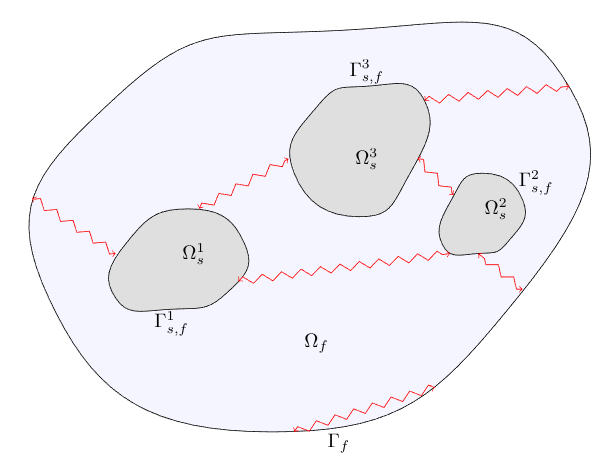
\includegraphics[width=1\linewidth]{PICTURES/domaine.png}
    

    
\end{minipage}
\hfill
\begin{minipage}{0.4\linewidth}
    Notations :
    
    $\Omega_s^i$ les différents domaines solides.
    
    $\Omega_s$ le domaine fluide.
    
    $\Gamma^i_{s,f}$ l'interface entre le solide $i$ et le fluide.
    
    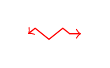
\begin{tikzpicture} 
        \draw[<->, red , decorate, decoration={zigzag, amplitude=2pt}]
        (0, 0) -- (0.67,0);
    \end{tikzpicture} Un symbole pour le couplage.
\end{minipage}
\caption{Schéma typique d’un problème de couplage conduction-rayonnement en milieu transparent}
\label{fig:domaine}
\end{figure}


Le problème revient à considérer l'équation de la chaleur dans les différents domaines.
Pour les solides :
\begin{equation}
    \forall i, \in \lbrace 1,2,3 \rbrace,\quad \forall \vec{r} \in  \Omega_s^i\quad \rho_s^i C_p^i \frac{\partial T(\vec{r})}{\partial t} =   -\lambda_{s}^i \Delta T(\vec{r}) + \dot{q}_{vol}(\vec{r})  
\end{equation}
Pour le fluide :
\begin{equation}
    \forall \vec{r}, \in  \Omega_s \quad \rho_f C_{p,f} \frac{\partial T(\vec{r})}{\partial t} =   -\lambda_f \Delta T(\vec{r}) + \dot{q}_{vol}(\vec{r})  
\end{equation}
Pour l'interface solide-fluide :
\begin{equation}
    \forall i, \in \lbrace 1,2,3 \rbrace,\quad \forall \vec{r} \in  \Gamma_s^i  , \left \lbrace
    \begin{array}{r c c c c}
      \vec{\phi}_s^i (\vec{r}) \cdot \vec{n}(\vec{r}) & = & \vec{\phi}_f (\vec{r}) \cdot \vec{n}(\vec{r}) + q_r(\vec{r}) & ,\text{avec}  & \vec{\phi}^i = -\lambda^i_s \nabla(T) \\
      T_s(\vec{r}) & = & T_f(\vec{r}) & 
    \end{array}\right.
\end{equation}

L'absence de terme source permet de trouver facilement l'allure de la température pour des géométries simples. On obtient en effet un profil linéaire (resp. logarithmique) en cartésien (resp. cylindrique).

\subsubsection{Premiers résultats du couplage en 2D avec \ttt{TrioCFD}}
Dans cet exemple précis, la solution de l'équation de la chaleur converge vers le résultat attendu. On peut extraire de \ttt{TrioCFD} les Figures \ref{fig:maillage2D} et \ref{fig:plot2D} qui montrent le bon accord de la simulation avec la théorie.

\begin{figure}[H]
\begin{minipage}{0.49\linewidth}

    \centering
    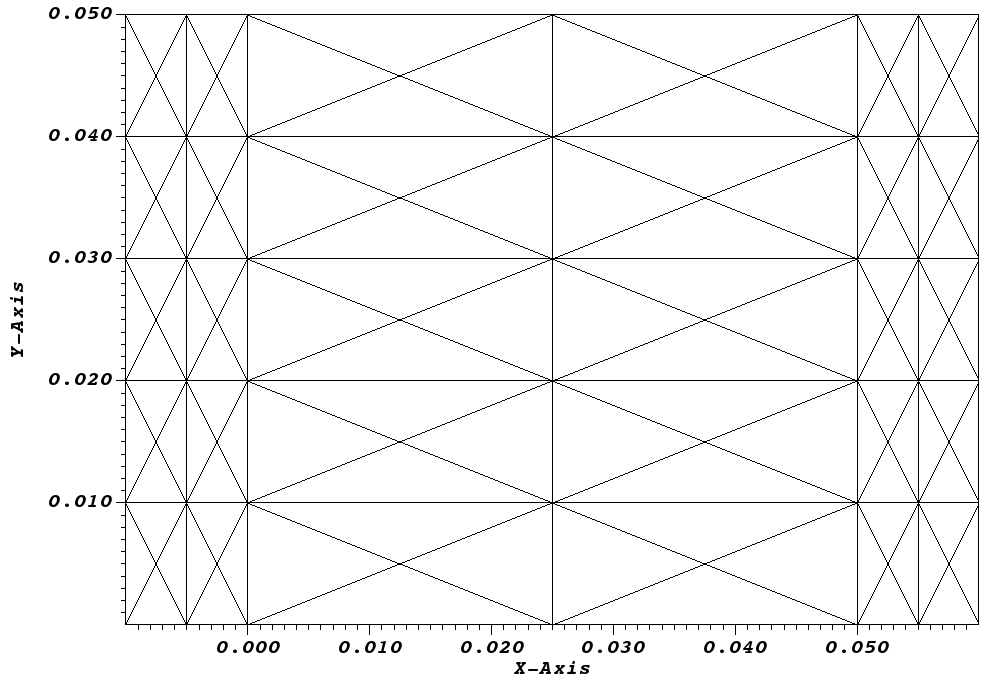
\includegraphics[width = \linewidth]{PICTURES/2D_VEF.png}
    \caption{Maillage pour la simulation en 2D}
    \label{fig:maillage2D}
\end{minipage}
\hfill
\begin{minipage}{0.49\linewidth}

    \centering
    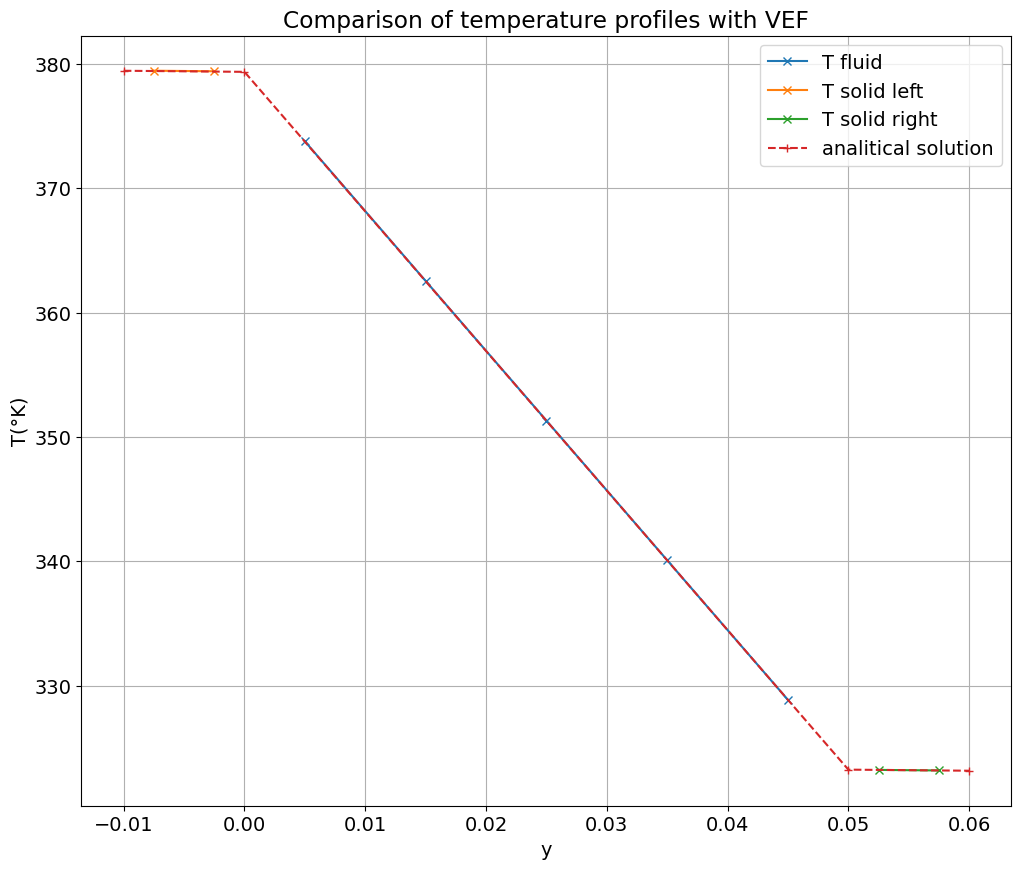
\includegraphics[width = 0.9\linewidth]{PICTURES/2D_VEF_plot.png}
    \caption{Courbe de température pour la simulation 2D}
    \label{fig:plot2D}
\end{minipage}
\end{figure}

La même conclusion est dressée pour une géométrie 3D ou cylindrique. L'important est plutôt de montrer que le module de rayonnement en milieu transparent de \ttt{TrioCFD} est fonctionnel. Par ailleurs, un travail d'amélioration d'une fiche de validation sur ce module de couplage est attendu.


\subsection{Combinaison \ttt{embree2TRUST} et \ttt{TrioCFD}}
Alors que la section précédente montre un bon accord entre la simulation couplée et le résultat attendu, la simulation faite dans \cite{lorenzo} (le travail de Lorezno) montre des écarts avec la simulation de \cite{Romain25} (code de référence). Il est intéressant de noter que la principale différence entre les deux simulations vient de la génération des facteurs de vue. Un travail plus approndi de vérification et validation du code \ttt{embree2TRUST} est donc attendu pour le stage.


